
\section{Histogram computation}

A histogram succinctly and meaningfully summarizes the data, thus histogram computation is a very
common analysis task. In this section, we study bit streams that aim to reproduce the most accurate
histogram possible at any bit rate. To do so, it is necessary to first define a criteria to compare
two histograms. In the literature, there have been many distance metric proposed for histograms;
among the more common ones are Bhattacharyya [CITE], Chi-square [CITE], Earth mover distance [CITe],
Kolmogorov-Smirnov [CITE], an Kullback-Liebler [CITE]. We use Algorithm [REF] to produce one stream
for each of these metrics and plot them against one another with PSNR as the metric (Figure [REF]).

\begin{figure}
	\centering
	\subcaptionbox{\emph{boiler}}
	{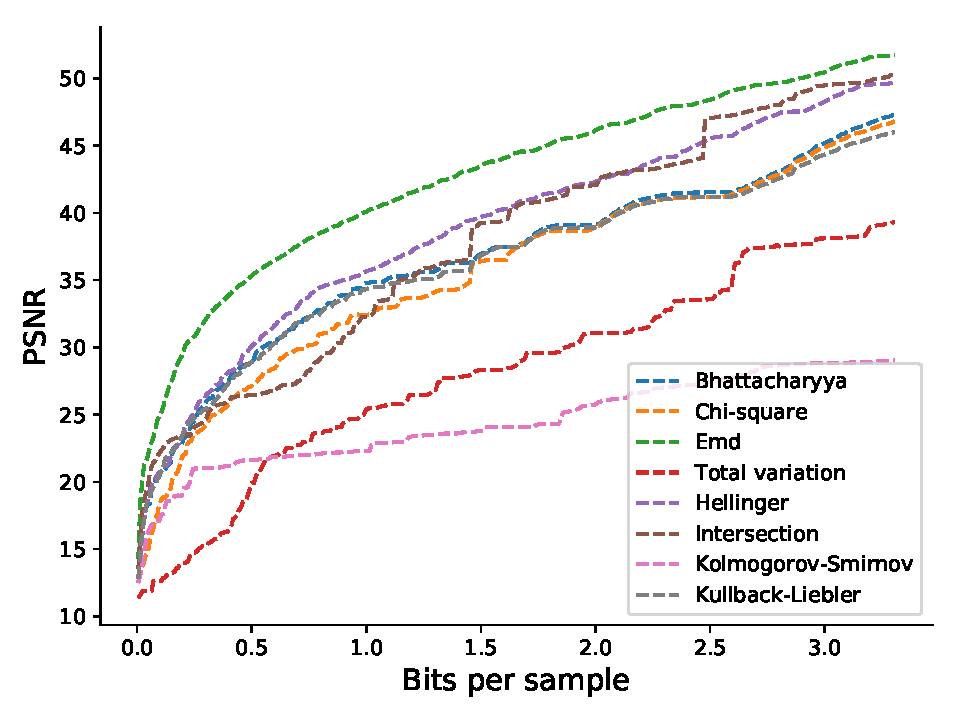
\includegraphics[width=0.48\linewidth]{img/histogram/different-metrics/boiler-histogram-metrics.pdf}}
	\subcaptionbox{\emph{kflame}}
	{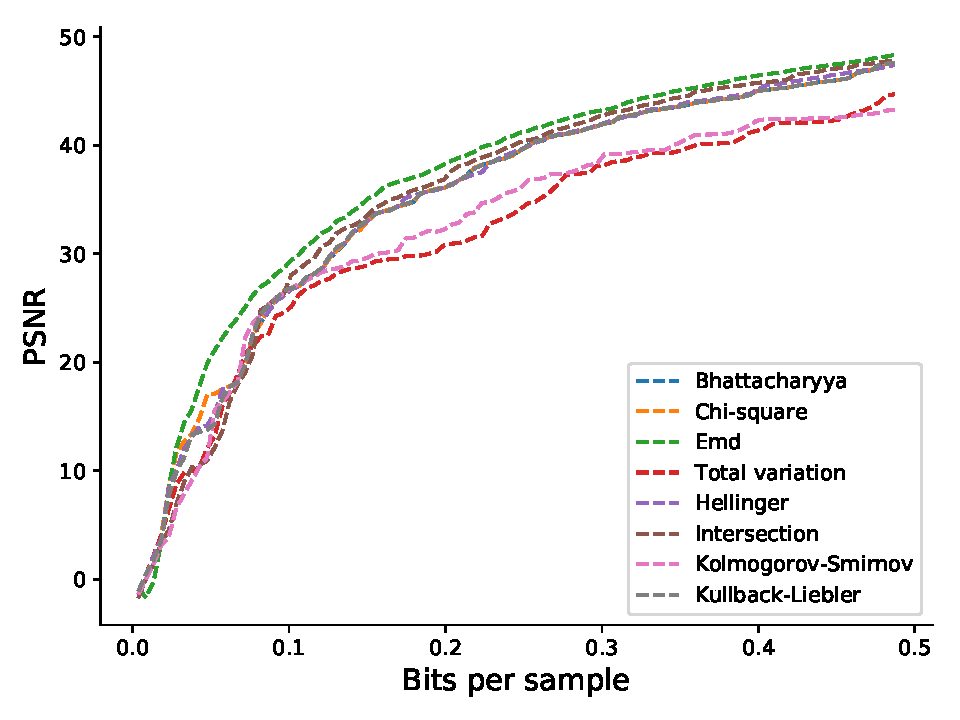
\includegraphics[width=0.48\linewidth]{img/histogram/different-metrics/kflame-histogram-metrics.pdf}}
	\subcaptionbox{\emph{diffusivity}}
	{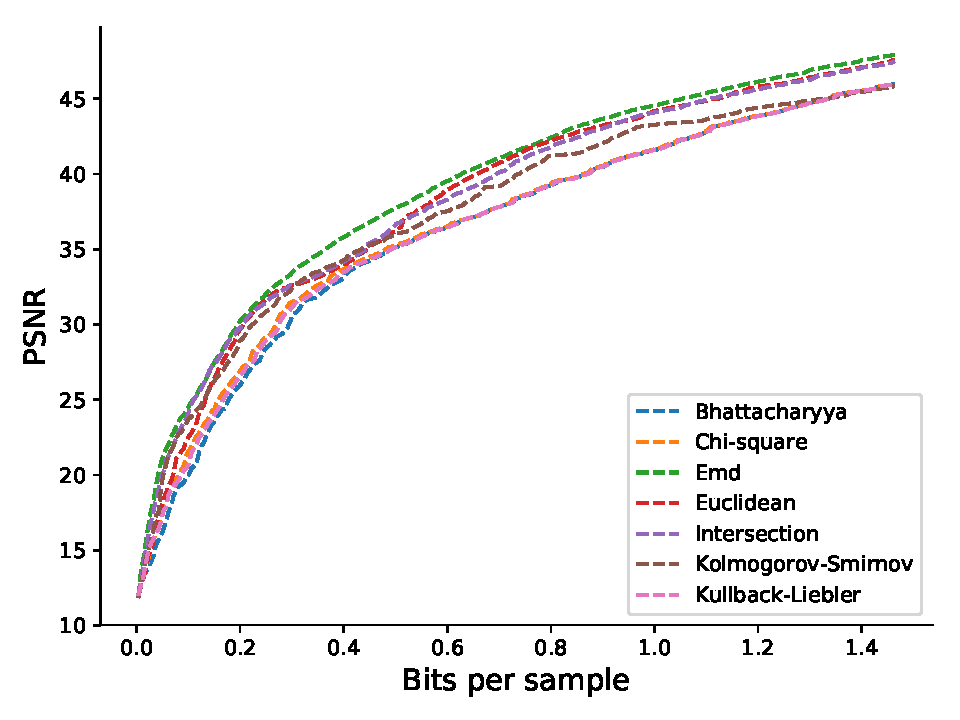
\includegraphics[width=0.48\linewidth]{img/histogram/different-metrics/miranda-diffusivity-histogram-metrics.pdf}}
	\subcaptionbox{\emph{turbulence}}
	{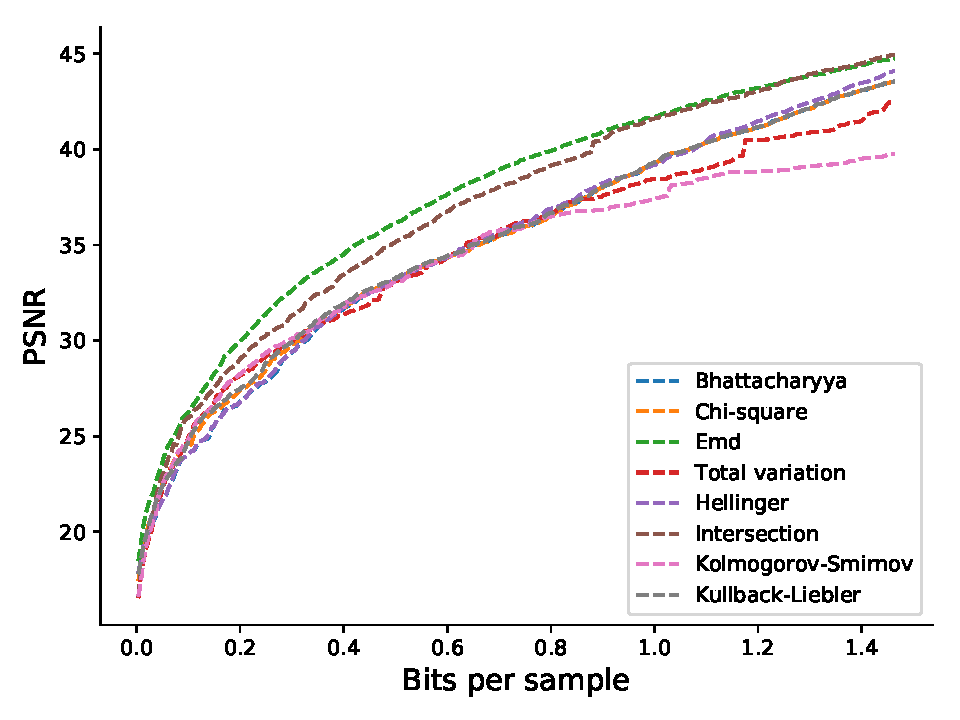
\includegraphics[width=0.48\linewidth]{img/histogram/different-metrics/turbulence-histogram-metrics.pdf}}
	\caption{Histogram comparison.}
	\label{fig:histogram-metrics-comparison}
\end{figure}

\begin{figure}
	\centering
	\subcaptionbox{\emph{bhattacharyya}}
	{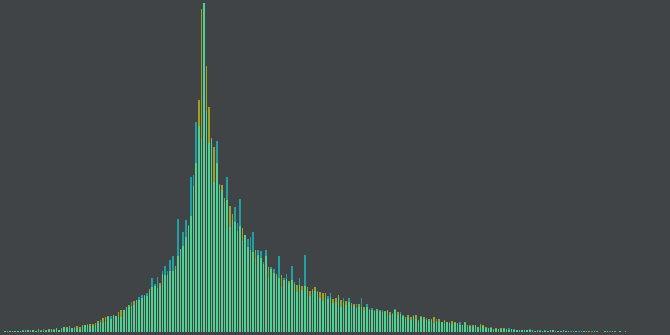
\includegraphics[width=0.48\linewidth]{img/histogram/different-metrics/bhattacharyya.png}}
	\subcaptionbox{\emph{chi-square}}
	{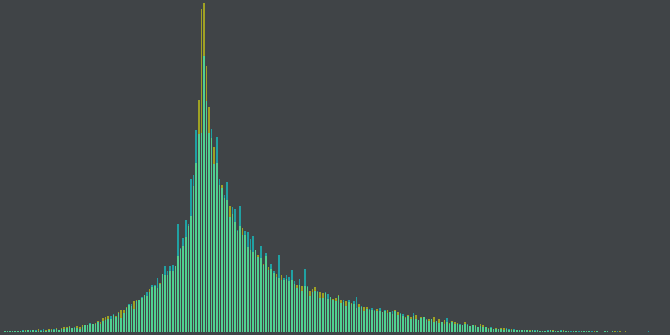
\includegraphics[width=0.48\linewidth]{img/histogram/different-metrics/chi_square.png}}
	\subcaptionbox{\emph{emd}}
	{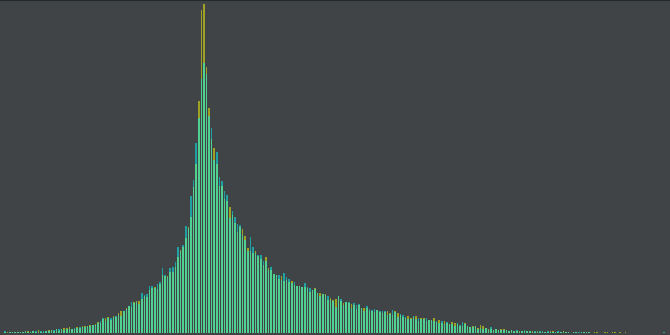
\includegraphics[width=0.48\linewidth]{img/histogram/different-metrics/emd.png}}
	\subcaptionbox{\emph{euclidean}}
	{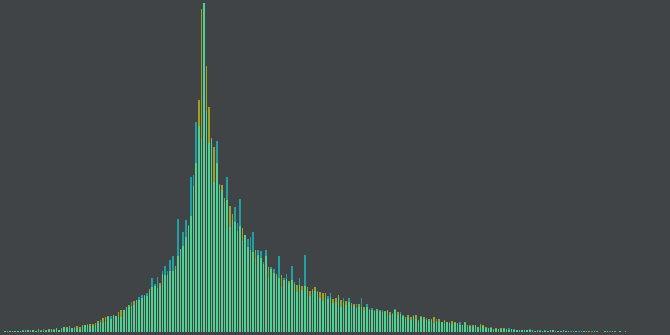
\includegraphics[width=0.48\linewidth]{img/histogram/different-metrics/euclidean.png}}
	\subcaptionbox{\emph{intersection}}
	{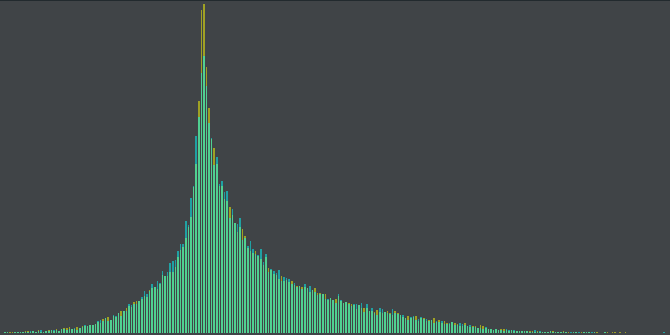
\includegraphics[width=0.48\linewidth]{img/histogram/different-metrics/intersection.png}}
	\subcaptionbox{\emph{kolmogorov-smirnov}}
	{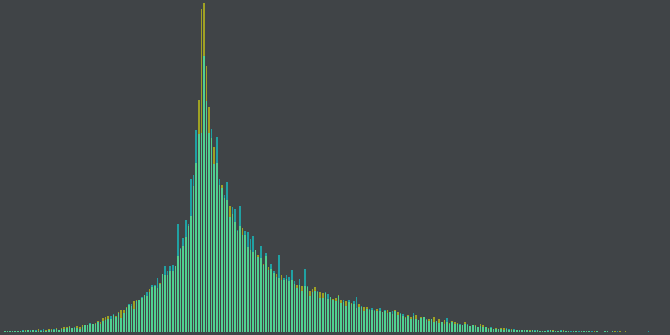
\includegraphics[width=0.48\linewidth]{img/histogram/different-metrics/kolmogorov_smirnov.png}}
	\subcaptionbox{\emph{kullback-liebler}}
	{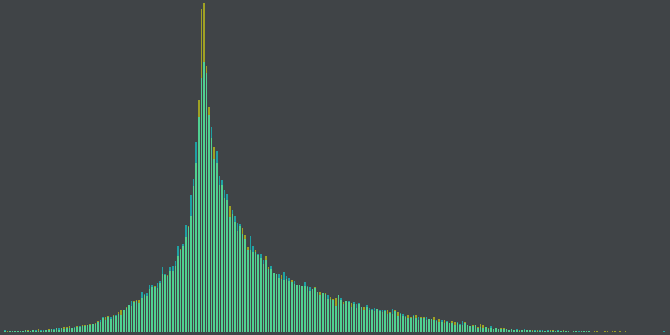
\includegraphics[width=0.48\linewidth]{img/histogram/different-metrics/kullback_liebler.png}}
	\caption{Histogram metrics comparison.}
	\label{fig:ahistogram-metrics-comparison}
\end{figure}

\begin{figure}
	\centering
	\subcaptionbox{\emph{boiler}}
	{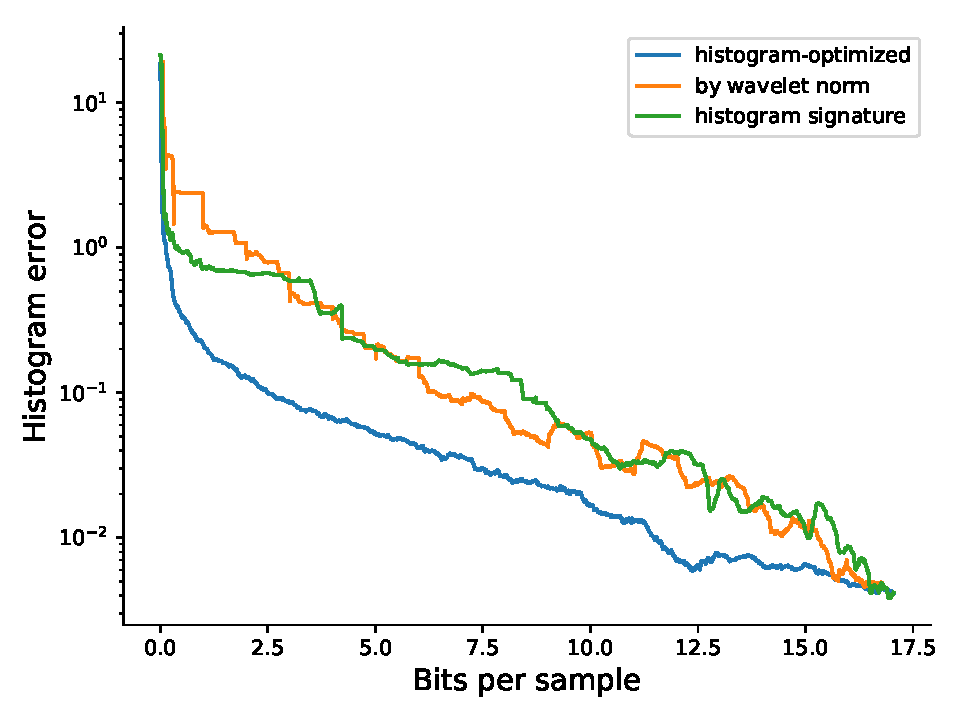
\includegraphics[width=0.48\linewidth]{img/histogram/boiler-histogram.pdf}}
	\subcaptionbox{\emph{boiler, slz}}
	{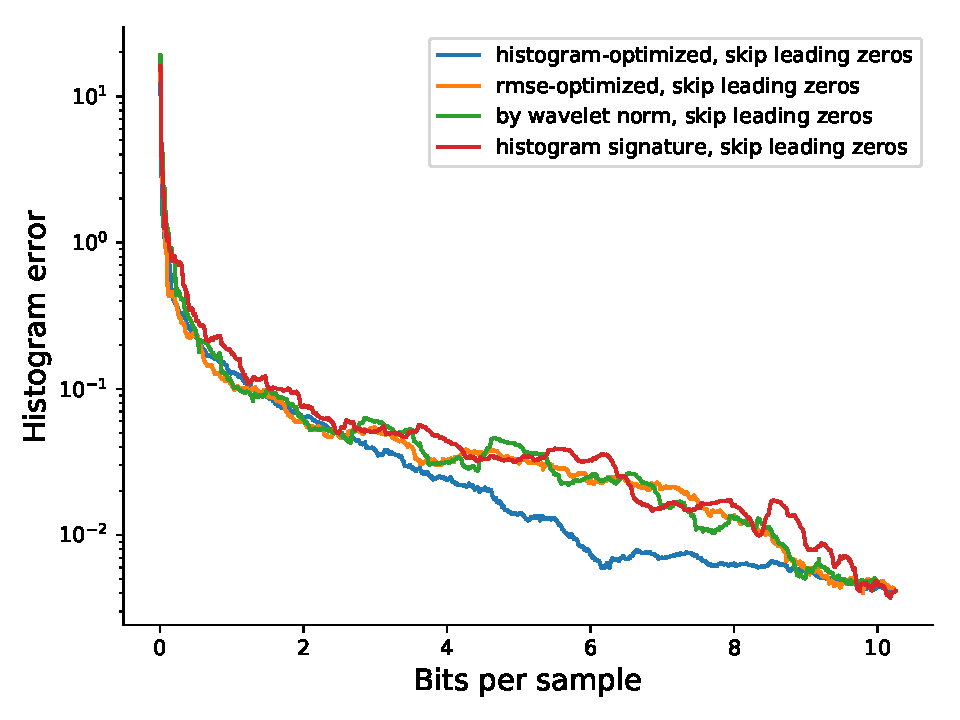
\includegraphics[width=0.48\linewidth]{img/histogram/skip-leading-zeros/boiler-histogram.pdf}}
	\subcaptionbox{\emph{kflame}}
	{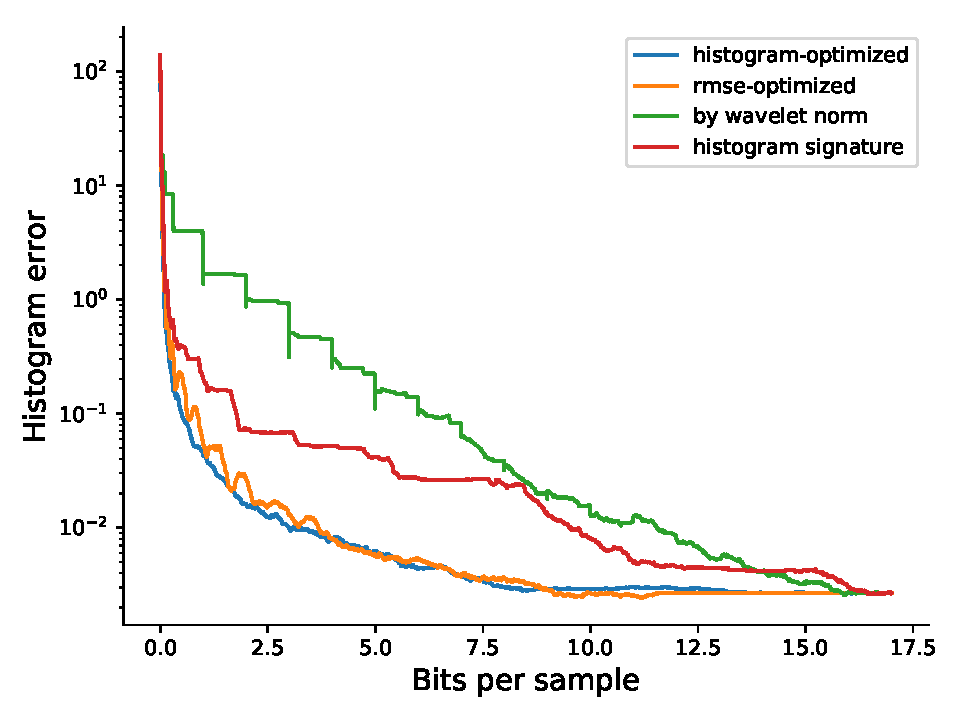
\includegraphics[width=0.48\linewidth]{img/histogram/kflame-histogram.pdf}}
	\subcaptionbox{\emph{kflame, slz}}
	{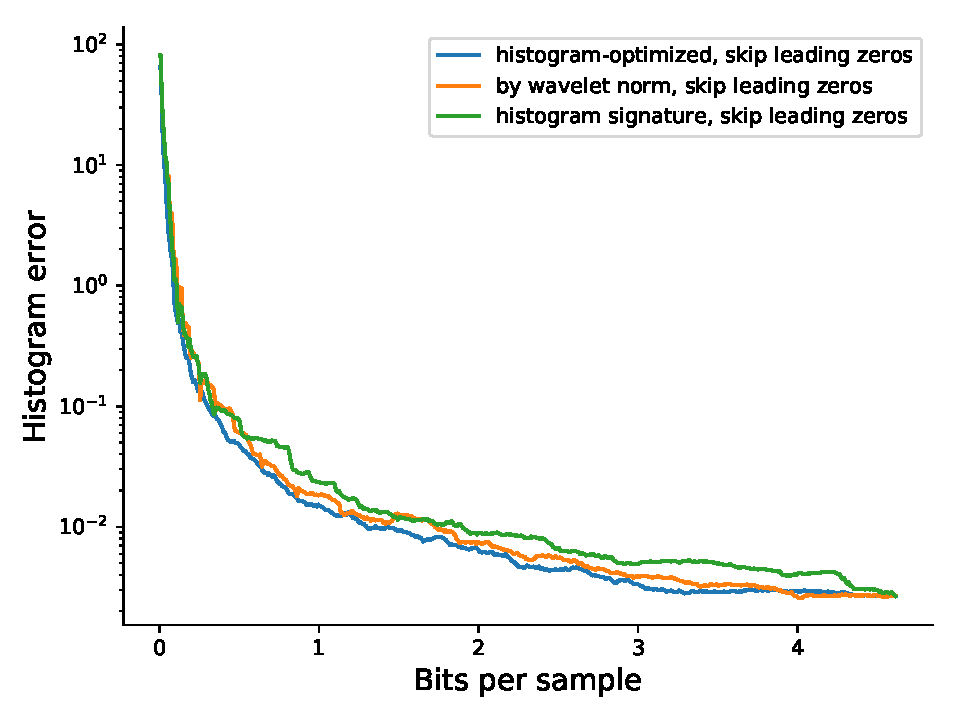
\includegraphics[width=0.48\linewidth]{img/histogram/skip-leading-zeros/kflame-histogram.pdf}}
	\subcaptionbox{\emph{diffusivity}}
	{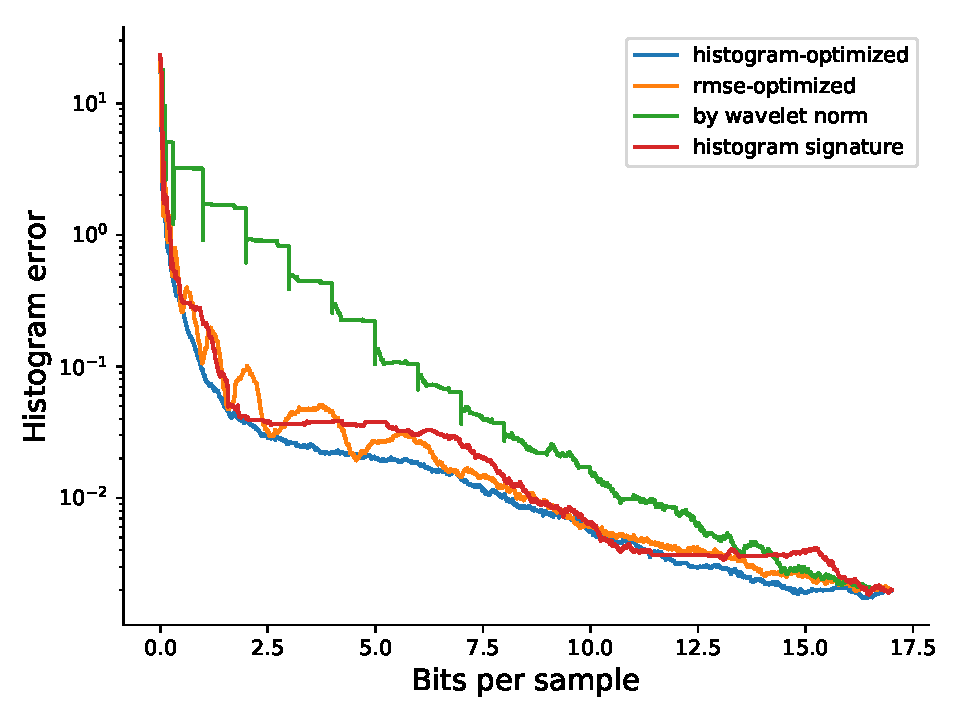
\includegraphics[width=0.48\linewidth]{img/histogram/miranda-diffusivity-histogram.pdf}}
	\subcaptionbox{\emph{diffusivity, slz}}
	{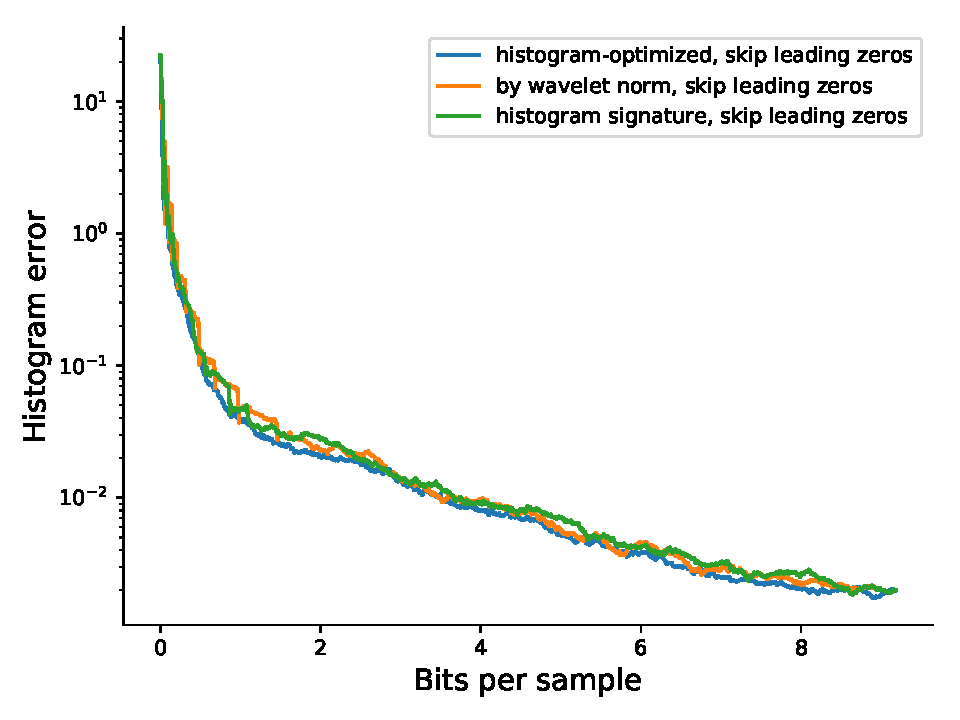
\includegraphics[width=0.48\linewidth]{img/histogram/skip-leading-zeros/miranda-diffusivity-histogram.pdf}}
	\subcaptionbox{\emph{turbulence}}
	{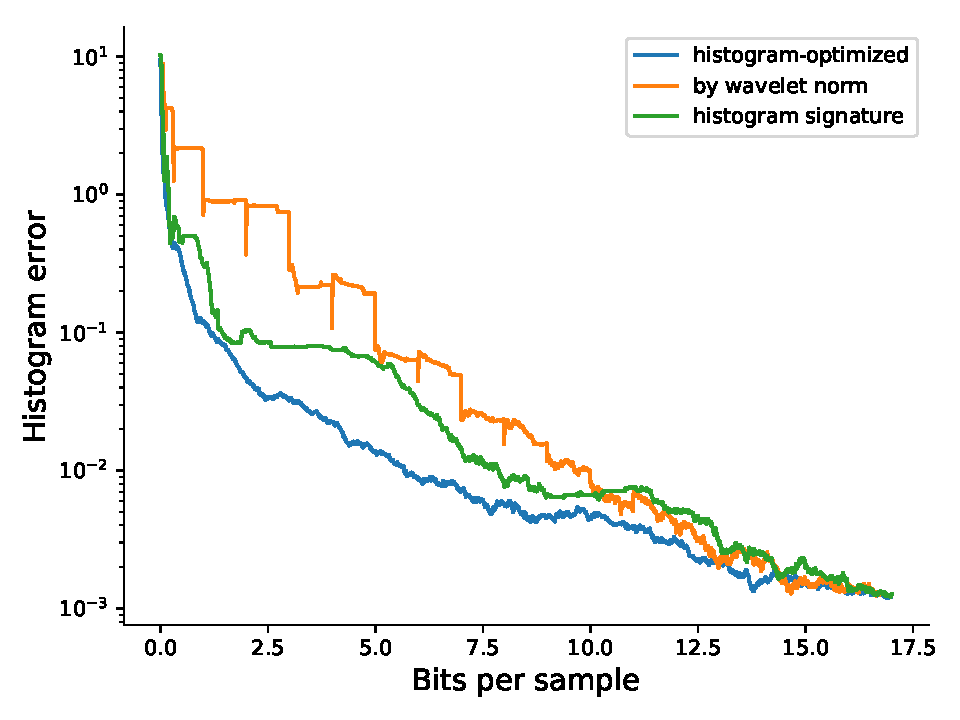
\includegraphics[width=0.48\linewidth]{img/histogram/turbulence-histogram.pdf}}
	\subcaptionbox{\emph{turbulence, slz}}
	{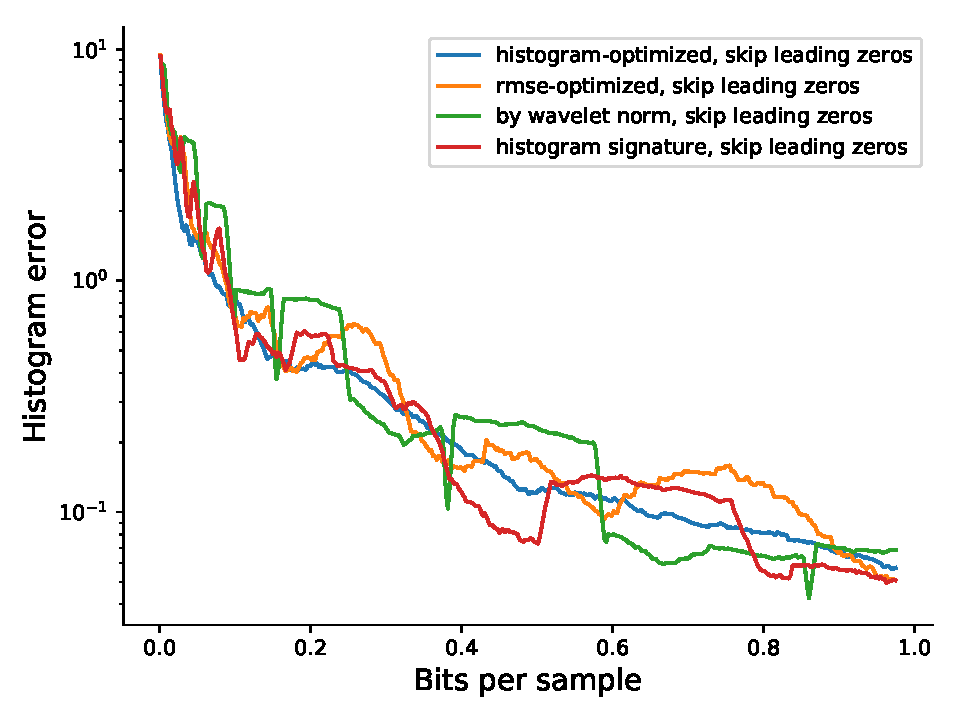
\includegraphics[width=0.48\linewidth]{img/histogram/skip-leading-zeros/turbulence-histogram.pdf}}
	\caption{Histogram comparison.}
	\label{fig:histogram-comparison}
\end{figure}

\begin{figure}
	\centering
	\subcaptionbox{\emph{histogram-optimized}}
	{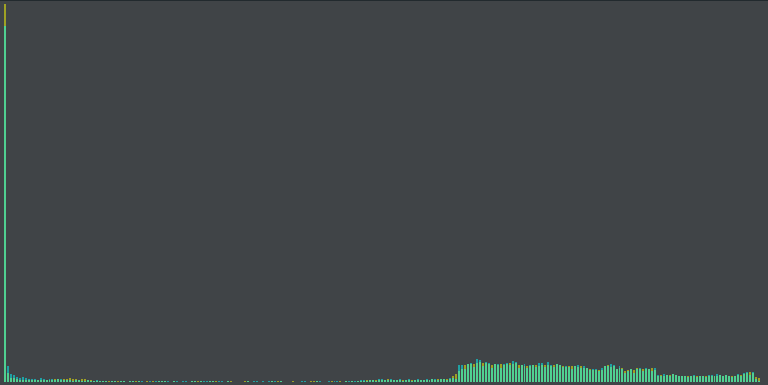
\includegraphics[width=0.24\linewidth]{img/histogram/kflame-wlz/histogram.png}}
	\subcaptionbox{\emph{rmse-optimized}}
	{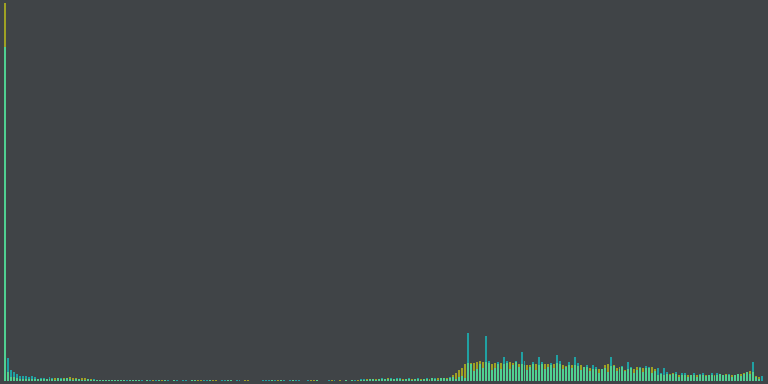
\includegraphics[width=0.24\linewidth]{img/histogram/kflame-wlz/rmse.png}}
	\subcaptionbox{\emph{by wavelet norm}}
	{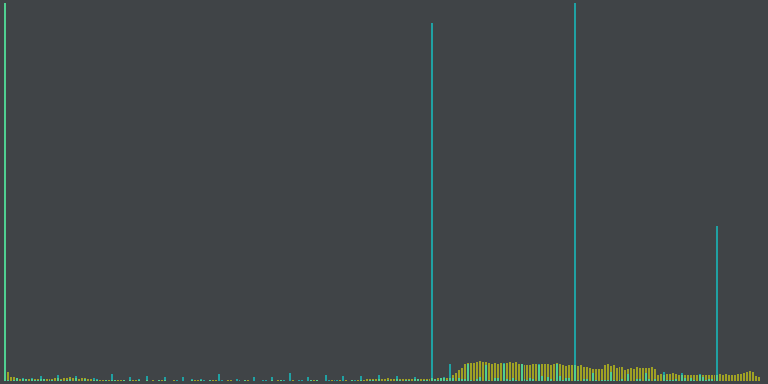
\includegraphics[width=0.24\linewidth]{img/histogram/kflame-wlz/wavenorm.png}}
	\subcaptionbox{\emph{histogram signature}}
	{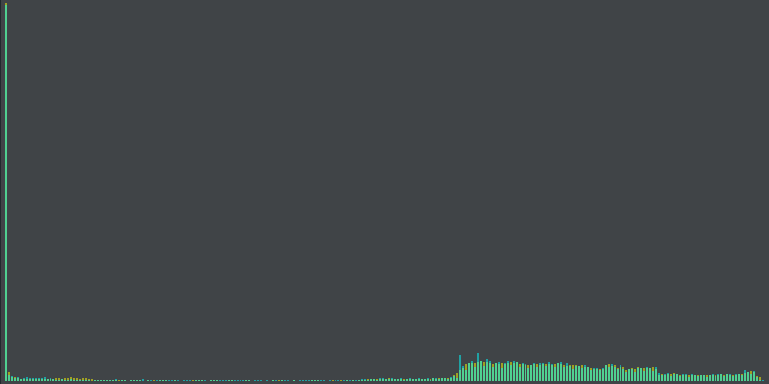
\includegraphics[width=0.24\linewidth]{img/histogram/kflame-wlz/signature.png}}
	\subcaptionbox{\emph{histogram-optimized}}
	{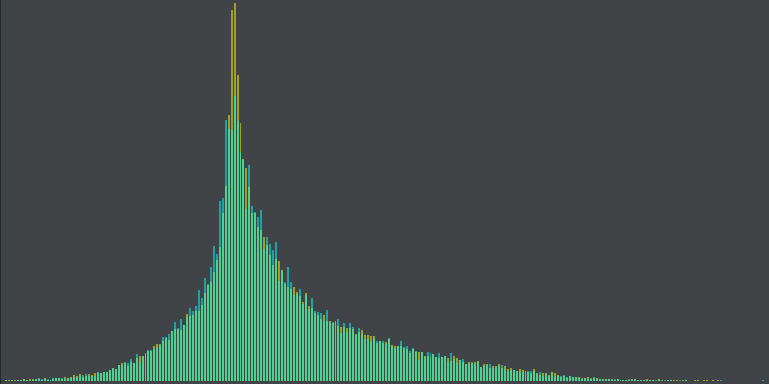
\includegraphics[width=0.24\linewidth]{img/histogram/diffusivity-wlz/histogram.png}}
	\subcaptionbox{\emph{rmse-optimized}}
	{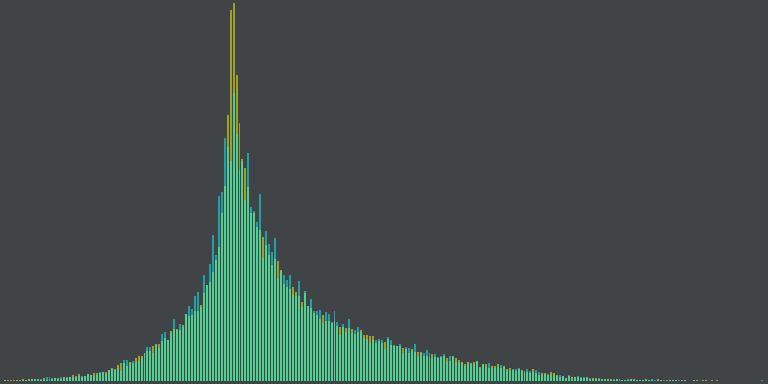
\includegraphics[width=0.24\linewidth]{img/histogram/diffusivity-wlz/rmse.png}}
	\subcaptionbox{\emph{by wavelet norm}}
	{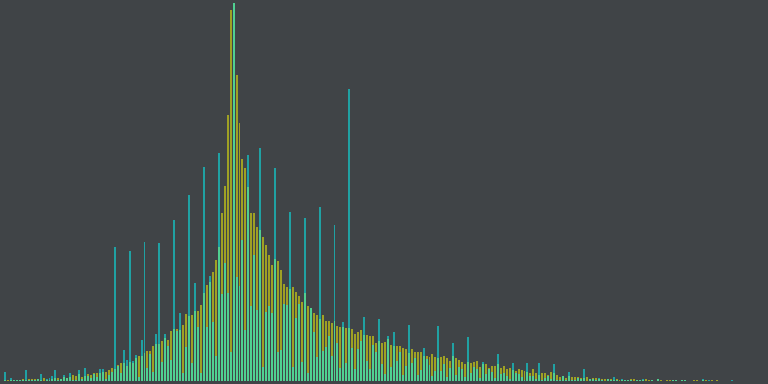
\includegraphics[width=0.24\linewidth]{img/histogram/diffusivity-wlz/wavenorm.png}}
	\subcaptionbox{\emph{histogram signature}}
	{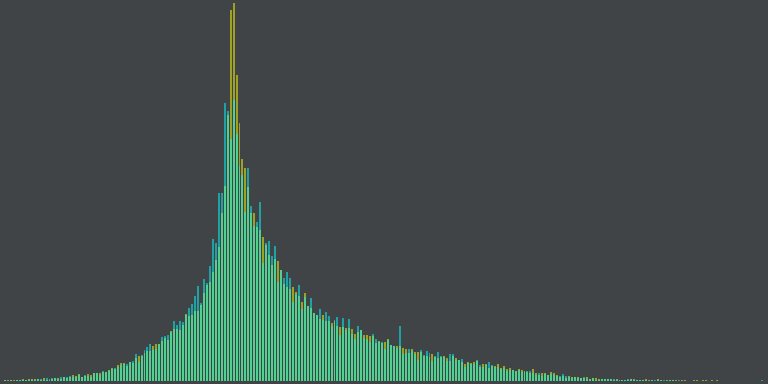
\includegraphics[width=0.24\linewidth]{img/histogram/diffusivity-wlz/signature.png}}
	\caption{Histogram comparison. (a,b,c,d) kflame, 0.17 bps. (e,f,g,h) diffusivity, 0.3 bps.}
	\label{fig:histogram-comparison-low-bit-rate}
\end{figure}

\begin{figure}
	\centering
	\subcaptionbox{\emph{histogram-optimized, slz}}
	{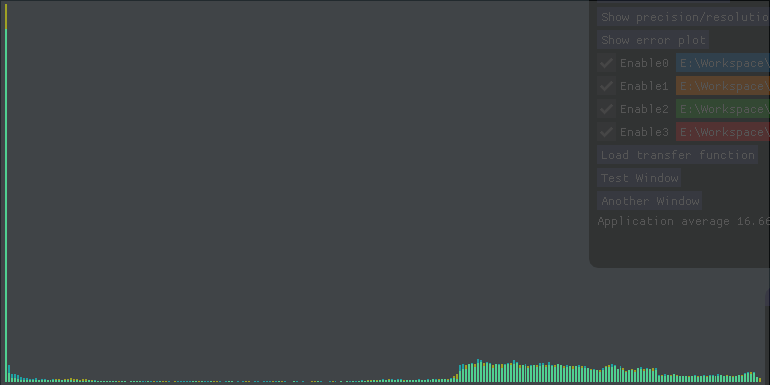
\includegraphics[width=0.24\linewidth]{img/histogram/kflame/histogram.png}}
	\subcaptionbox{\emph{rmse-optimized, slz}}
	{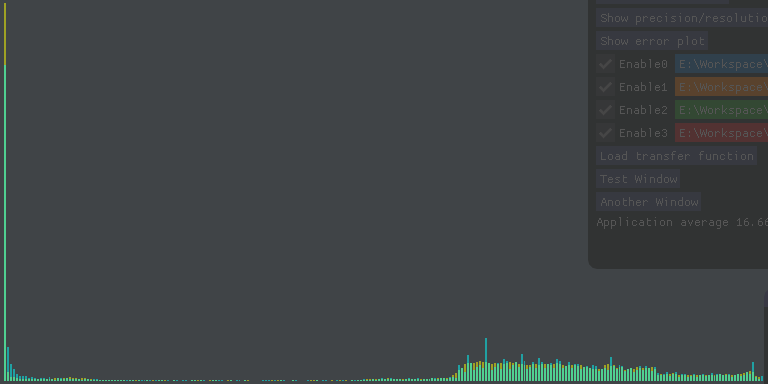
\includegraphics[width=0.24\linewidth]{img/histogram/kflame/rmse.png}}
	\subcaptionbox{\emph{by wavelet norm, slz}}
	{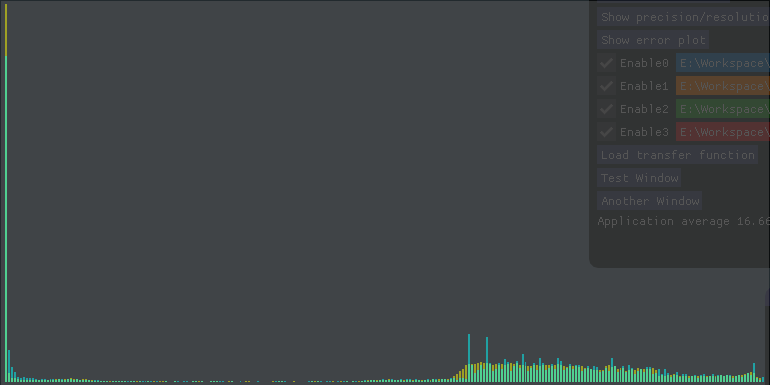
\includegraphics[width=0.24\linewidth]{img/histogram/kflame/wavenorm.png}}
	\subcaptionbox{\emph{histogram signature, slz}}
	{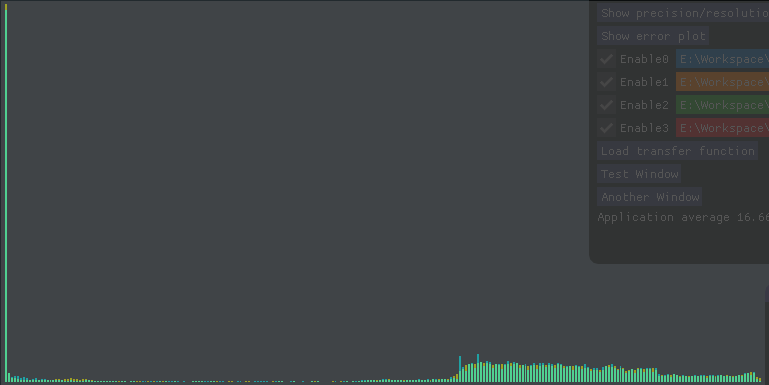
\includegraphics[width=0.24\linewidth]{img/histogram/kflame/signature.png}}
	\subcaptionbox{\emph{histogram-optimized, slz}}
	{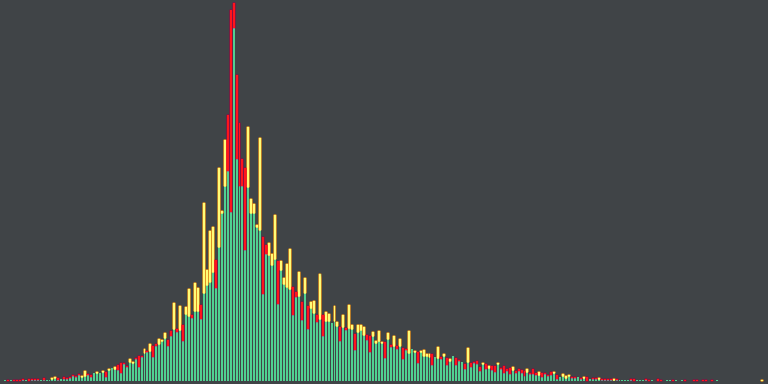
\includegraphics[width=0.24\linewidth]{img/histogram/diffusivity/histogram.png}}
	\subcaptionbox{\emph{rmse-optimized, slz}}
	{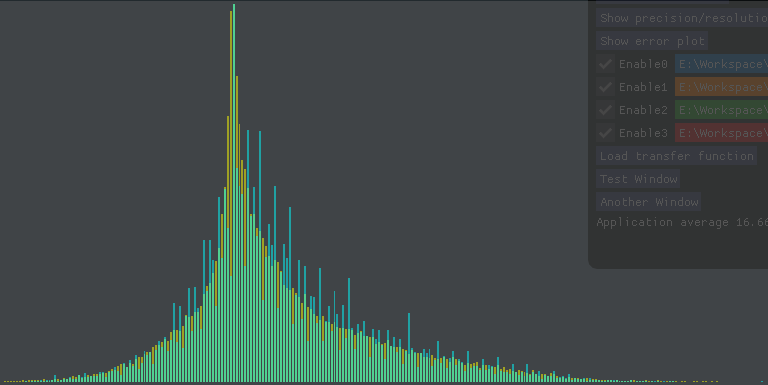
\includegraphics[width=0.24\linewidth]{img/histogram/diffusivity/rmse.png}}
	\subcaptionbox{\emph{by wavelet norm, slz}}
	{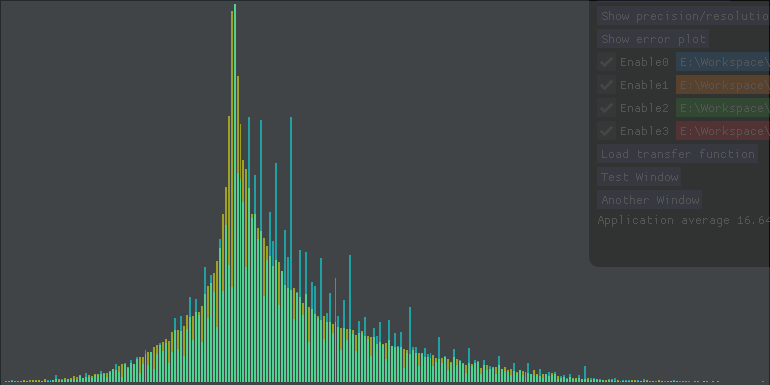
\includegraphics[width=0.24\linewidth]{img/histogram/diffusivity/wavenorm.png}}
	\subcaptionbox{\emph{histogram signature, slz}}
	{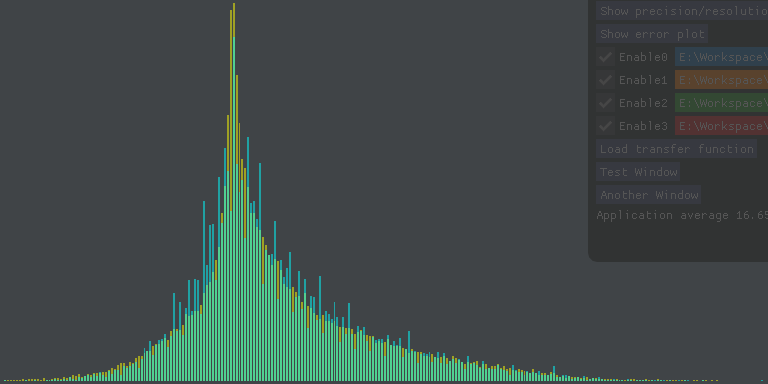
\includegraphics[width=0.24\linewidth]{img/histogram/diffusivity/signature.png}}
	\caption{Histogram comparison at low bit rates, using skip-leading-zeros. (a,b,c,d) kflame, 0.14 bps. (e,f,g,h) diffusivity, 0.09 bps.}
	\label{fig:histogram-comparison-low-bit-rate}
\end{figure}

Histogram computation is another common 
We compare different error metric for histogram in two figures:
Figure 1: PSNR plot for all histogram streams using different error metrics.

Figure 2: histogram plots for each metric, at some low bit rate

Figure 3: RMSE error between rmse stream and histogram stream for one data set

Figure 4: Histogram error for the  above two streams for the same data set.

To somewhat quantify the differences of two streams, we define the concept of a stream signature, and present the algorithm to compute a signature.

Algorithm. How to compute a stream's signature.

We show the two signatures for rmse and histogram streams for the same data set.

Figure 5: show signature of the two streams

Figure 6: show signatures for different number of bins

Figure 7: Show that we can stream using the histogram signature to get better histogram than rmse